\documentclass[oneside,a4paper,german,parskip=half,draft]{scrbook}

\usepackage[latin1]{inputenc}

%Neue Deutsche Rechtschreibung
\usepackage{ngerman}

%Seitenheader
\usepackage{fancyhdr}
\pagestyle{fancy}
\rhead{\nouppercase{\rightmark}}
\lhead{\nouppercase{\leftmark}}

%Standartfont
\usepackage[T1]{fontenc}
%\usepackage{fourier}
%\usepackage{libertine}

%Zusatzpaket f�r mathematische Ausdr�cke
\usepackage{amsmath}

%Zusatzfonts f�r mathbb usw.
\usepackage{amsfonts}
\usepackage{mathrsfs}

%Verbessertes Ref
\usepackage[german]{varioref}

%Links
\usepackage{hyperref}

%Stichwortverzeichnis
\usepackage{makeidx}
\makeindex

%Acronyme
\usepackage[nolist,nohyperlinks]{acronym}

%Anpassbare Enumerates/Itemizes
\usepackage{enumitem}

%Tikz/PGF Zeichnenpaket
\usepackage{pgf}
\usepackage{tikz}
\usetikzlibrary{mindmap,trees,decorations,decorations.pathreplacing,decorations.pathmorphing,calc,arrows,automata}

%F�r graphische Todos
\usepackage[colorinlistoftodos, obeyDraft]{todonotes}

%Paket zum Berechnen von Textbreiten und H�hen
\usepackage{calc}

%BibTeX
%\usepackage{cite}
%\usepackage{bibgerm}
%\bibliographystyle{gerplain}

%F�r das manipulieren von Captions in Figuren
\usepackage{caption}

%F�r das anpassen von theoremen
\usepackage{amsthm}

%F�r die farbigen Boxen
\usepackage{xcolor}
\usepackage{framed}

%Um die Seite in mehrere Spalten aufzuteilen
\usepackage{multicol}

%F�r zwischenr�ume in W�rtern
\usepackage{xspace}

%Quellcode Einbindung
\usepackage{listings}
\lstset{
basicstyle=\ttfamily
}

%F�r das durchstreichen von Bl�cken
\usepackage{cancel}

%F�r Commandos mit zwei opotionalen Argumenten
\usepackage{twoopt}

% \if\blank --- checks if parameter is blank (Spaces count as blank) 
% \if\given --- checks if parameter is not blank: like \if\blank{#1}\else 
% \if\nil --- checks if parameter is null (spaces are NOT null) 
% use \if\given{ } ... \else ... \fi etc. 
% Beispiel: \newcommand{\blah}[1]{\if\blank{#1}Leer\else#1\fi}
% 
{\catcode`\!=8 % funny catcode so ! will be a delimiter 
\catcode`\Q=3 % funny catcode so Q will be a delimiter 
\long\gdef\given#1{88\fi\Ifbl@nk#1QQQ\empty!} 
\long\gdef\blank#1{88\fi\Ifbl@nk#1QQ..!}% if null or spaces 
\long\gdef\nil#1{\IfN@Ught#1* {#1}!}% if null 
\long\gdef\IfN@Ught#1 #2!{\blank{#2}} 
\long\gdef\Ifbl@nk#1#2Q#3!{\ifx#3}% same as above 
}

%<Commandos>
%In geschweifte Klammern setzen
\newcommand{\gklamm}[1]{\ensuremath{\left\{#1\right\}}}

%In eckige Klammern setzen
\newcommand{\eklamm}[1]{\ensuremath{\left[#1\right]}}

%In runde Klammern setzen
\newcommand{\rklamm}[1]{\ensuremath{\left(#1\right)}}

%In Betragsstriche Setzen
\newcommand{\betrag}[1]{\ensuremath{\left|#1\right|}}

%Script zum Eingeben von l�ngeren Beispielen
\newcommand{\bsp}[3][]
{
\if\blank{#3}\textalign{\textbf{#2}}{#1}\else
\textbf{#2} #1
\par
\begingroup
\leftskip=1.28em
\setlist[1]{labelindent=1.28em, leftmargin=*}
#3
\par
\endgroup\fi
}

%Script um Text einzur�cken
\newcommand{\textalign}[2]{
\begin{minipage}[b]{\widthof{#1} + \widthof{\space}}
#1
\end{minipage}
\begin{minipage}[t]{\linewidth-\widthof{#1}-\widthof{\space}}
#2
\end{minipage}
}

%Script um Text einzur�cken ohne Ausgabe
\newcommand{\textfakealign}[3]{
\begin{minipage}[b]{\widthof{#1} + \widthof{\space}}
\if\blank{#2}$ $\else#2\fi
\end{minipage}
\begin{minipage}[t]{\linewidth-\widthof{#1}-\widthof{\space}}
#3
\end{minipage}
}

%Indexe
%Normaler Index
\newcommand{\indexn}[2][]{#2\if\blank{#1}\index{#2}\else\index{#1}\fi}
%Unterstrichener Index
\newcommand{\indexu}[2][]{\underline{#2}\if\blank{#1}\index{#2}\else\index{#1}\fi}
%Kursiver Index
\newcommand{\indexi}[2][]{\textit{#2}\if\blank{#1}\index{#2}\else\index{#1}\fi}
%Fetter Index
\newcommand{\indexb}[2][]{\textbf{#2}\if\blank{#1}\index{#2}\else\index{#1}\fi}

%Definitionen, Beispiele, S�tze
\newenvironment{fshaded}[2]{%
\def\FrameCommand{\fcolorbox{#1}{#2}}%
\MakeFramed {\FrameRestore}}%
{\endMakeFramed}

\theoremstyle{definition}
\newtheorem{definition}{\ac{Def.}}[part]
\newenvironment{fdefinition}[1][]{\definecolor{shadecolor_definition}{rgb}{.87,.94,.96}
\definecolor{framecolor_definition}{rgb}{0,0,0}%
\begin{fshaded}{framecolor_definition}{shadecolor_definition}\begin{definition}[#1]}{\end{definition}\end{fshaded}}

\newtheorem{satz}[definition]{Satz}
\newenvironment{fsatz}[1][]{\definecolor{shadecolor_satz}{rgb}{.87,.96,.56}
\definecolor{framecolor_satz}{rgb}{0,0,0}%
\begin{fshaded}{framecolor_satz}{shadecolor_satz}\begin{satz}[#1]}{\end{satz}\end{fshaded}}

\newtheorem{beweis}{Beweis}[part]
\newenvironment{fbeweis}[1][]{\definecolor{shadecolor_beweis}{rgb}{1.00,.96,.92}
\definecolor{framecolor_beweis}{rgb}{0,0,0}%
\begin{fshaded}{framecolor_beweis}{shadecolor_beweis}\begin{beweis}[#1]}{\end{beweis}\end{fshaded}}

\theoremstyle{remark}
\newtheorem{notation}{Notation}[part]
\newenvironment{fnotation}[1][]{\definecolor{shadecolor_notation}{rgb}{.90, .90, .90}
\definecolor{framecolor_notation}{rgb}{0,0,0}%
\begin{fshaded}{framecolor_notation}{shadecolor_notation}\begin{notation}[#1]}{\end{notation}\end{fshaded}}

\newtheoremstyle{note}% name
	{1em}			%Space above
	{1em}			%Space below
	{}				%Body font
	{}				%Indent amount (empty = no indent, \parindent = para indent)
	{\bfseries}	%Thm head font
	{:}			%Punctuation after thm head
	{.5em}		%Space after thm head: " " = normal interword space; \newline = linebreak
	{}				%Thm head spec (can be left empty, meaning `normal')

\newtheoremstyle{notelite}% name
	{3pt}			%Space above
	{3pt}			%Space below
	{}				%Body font
	{}				%Indent amount (empty = no indent, \parindent = para indent)
	{\itshape}	%Thm head font
	{:}			%Punctuation after thm head
	{.5em}		%Space after thm head: " " = normal interword space; \newline = linebreak
	{}				%Thm head spec (can be left empty, meaning `normal')

\theoremstyle{note}
\newtheorem*{beispiel}{Beispiel}

\theoremstyle{notelite}
\newtheorem*{anmerkung}{Anmerkung}
\newtheorem*{beobachtung}{Beobachtung}
\newtheorem*{bemerkung}{Bemerkung}
\newtheorem*{achtung}{Achtung}
%%%%%%%%Arabische in R�mische Zahl umwandeln
\newcommand{\RM}[1]{\ensuremath{\mbox{\MakeUppercase{\romannumeral #1}}}}
\newcommand{\rM}[1]{\ensuremath{\mbox{\romannumeral #1}}}
%</Commandos>

%<Abk�rzungen>
\newcommand{\Ra}{\ensuremath{\Rightarrow}}
\newcommand{\ra}{\ensuremath{\rightarrow}}
\newcommand{\La}{\ensuremath{\Leftarrow}}
\newcommand{\la}{\ensuremath{\leftarrow}}
\newcommand{\Ral}{\ensuremath{\Longrightarrow}}
\newcommand{\ral}{\ensuremath{\longrightarrow}}
\newcommand{\Lra}{\ensuremath{\Leftrightarrow}}
\newcommand{\lra}{\ensuremath{\leftrightarrow}}
\newcommand{\hra}{\ensuremath{\hookrightarrow}}
\newcommand{\mul}{\ensuremath{\cdot}}
\newcommand{\grgl}{\ensuremath{\geq}}
\newcommand{\klgl}{\ensuremath{\leq}}
\newcommand{\oder}{\ensuremath{\vee}}
\newcommand{\und}{\ensuremath{\wedge}}
\newcommand{\mal}{\ensuremath{\cdot}}
\newcommand{\matrixp}[1]{\ensuremath{\begin{pmatrix} #1 \end{pmatrix}}}
\newcommand{\coloneqq}{\mathrel{\mathop:\!\!=}}
\newcommand{\ceq}{\ensuremath{\coloneqq}}
\newcommand{\tx}[1]{\ensuremath{\text{#1}}}
\newcommand{\rkl}[1]{\ensuremath{\rklamm{#1}}}
\newcommand{\N}{\ensuremath{\mb{N}}}
\newcommand{\R}{\ensuremath{\mb{R}}}
\newcommand{\Z}{\ensuremath{\mb{Z}}}
\newcommand{\stack}[2]{\ensuremath{\stackrel{#1}{#2}}}
\newcommand{\ub}[2]{\ensuremath{\underbrace{#1}_{#2}}}

%Todo, Insert, Mark, Img
\newcommand{\Todo}[1]{\todo[inline]{TODO: #1}}
\newcommand{\Insert}[1]{\todo[inline, color=green!40]{INSERT: #1}}
\newcommand{\Mark}[1]{\todo[inline, nolist, color=blue!40]{MARK: #1}}
\newcommand{\Img}[1]{\todo[inline, nolist, color=black!40]{IMG: #1}}

%Sin, Cos, Tan, Dim, Span, Arccos, Limes
\DeclareMathOperator{\spano}{span}
\DeclareMathOperator{\lb}{lb}

\newcommand{\sinx}[1]{\ensuremath{\sin{\left(#1\right)}}}
\newcommand{\cosx}[1]{\ensuremath{\cos{\left(#1\right)}}}
\newcommand{\tanx}[1]{\ensuremath{\tan{\left(#1\right)}}}
\newcommand{\dimx}[1]{\ensuremath{\dim{\left(#1\right)}}}
\newcommand{\spanx}[1]{\ensuremath{\spano{\left(#1\right)}}}
\newcommand{\arccosx}[1]{\ensuremath{\arccos{\left(#1\right)}}}

%Schriften
\newcommand{\mb}[1]{\ensuremath{\mathbb{#1}}}
%</Abk�rzungen>




%<Einstellung f�r Hyperref>%%%%%%%%%%%%%%%%%%%%%%%%%%%%%%%%%%%%%%%%%%%%%%%%%%%%
\hypersetup{colorlinks=false, linkcolor=black, breaklinks=true, bookmarksdepth=3,unicode=true,bookmarksnumbered=true,
pdftitle={Hefter f�r Grundlagen der Informatik-- Stand: \today},
pdfauthor={Thaller Alexander},
pdfsubject={Hefter f�r das Fach Grundlagen der Informatik aus der Vorlesung von Professor Dr. rer. nat. Jorg Striegnitz (Str) f�r das 2. Semester der Informatik im Sommersemester 2009 an der Hochschule Regensburg.},
pdfkeywords={informatik,studium,hefter,gi,sommersemester,2009,grundlagen der informatik}}
%</Einstellung f�r Hyperref>%%%%%%%%%%%%%%%%%%%%%%%%%%%%%%%%%%%%%%%%%%%%%%%%%%%

%<Dokument Daten>%%%%%%%%%%%%%%%%%%%%%%%%%%%%%%%%%%%%%%%%%%%%%%%%%%%%%%%%%%%%%%
\titlehead{\includegraphics[width=34mm]{FH-Logo.pdf}}
\subject{Informatik (Bachelor) 2. Semester}
\author{Alexander Thaller}
\title{Grundlagen der Informatik\footnote{Gefundene Fehler oder Verbesserungsvorschlge bitte hier \href{http://fhrein2ss09.codeplex.com}{http://fhrein2ss09.codeplex.com/} berichten oder alternativ mir eine E-Mail schreiben \href{mailto:alexander.thaller@stud.fh-regensburg.de}{alexander.thaller@stud.fh-regensburg.de}. Vielen Dank.}}
\subtitle{Hefter des Sommersemesters 2009}
\date{stand \today}
\publishers{Aus der Vorlesung von Professor Dr. rer. nat. Jorg Striegnitz (Str)}
%</Dokument Daten>%%%%%%%%%%%%%%%%%%%%%%%%%%%%%%%%%%%%%%%%%%%%%%%%%%%%%%%%%%%%%
\begin{document}
\frontmatter
\begin{acronym}
	\acro{acr}{Akronym}
	\acro{zB}[\ensuremath{\mbox{z.\,B.}\xspace}]{zum Beispiel}
	\acro{bel.}{beliebigem}
	\acro{Def.}{Definition}
	\acro{gdw.}[\ensuremath{\mbox{g.\,d.\,w.}\xspace}]{genau dann wenn}
	\acro{def.}{definiert}
	\acro{Opt.}{Optimiert}
	\acro{DEA}{Deterministischer endlicher Automat}
	\acro{akzept.}{akzeptierende}
	\acro{bzw.}{beziehungsweise}
	\acro{bzgl.}{bez�glich}
	\acro{NEA}{Nichtdeterministische endliche Automaten}
	\acro{Ber.}{Berechnung}
	\acro{Berechn.}{Berechnung}
	\acro{Bew.}{Beweis}
	\acro{d.h}[\ensuremath{\mbox{d.\,h.}\xspace}]{daher}
	\acro{akz.}{akzeptierende}
	\acro{ex.}{existiert}
	\acro{Anw.}{Anwendung}
	\acro{M�gl.}{M�glichkeit}
\end{acronym}

\maketitle
\setcounter{tocdepth}{1}
\setcounter{secnumdepth}{3}
\clearpage
\pdfbookmark[0]{\contentsname}{tocanc}
\tableofcontents
\newpage
\listoftodos
\newpage
%<Text>%%%%%%%%%%%%%%%%%%%%%%%%%%%%%%%%%%%%%%%%%%%%%%%%%%%%%%%%%%%%%%%%%%%%%%%%
%\section*{�bersicht}
\begin{description}
\item[Professor:] Jorg Striegnitz
\item[Homepage:] \href{http://homepages.fh-regensburg.de/~stj39817/index.html}{http://homepages.fh-regensburg.de/~stj39817/index.html}
\item[E-Mail:] \href{mailto:joerg.striegnitz@informatik.fh-regensburg.de}{joerg.striegnitz@informatik.fh-regensburg.de}
\item[Zeitplan:]\mbox{}\par
		\begin{itemize}
		\item 4 Stunden pro Woche
		\item 2 Stunden Vorlesung
		\item 2 Stunden �bungen
		\end{itemize}
\item[Klausur:] Zulassungsvorrausetzungen: 50\% in den �bungen und eine Aufgabe Vorrechnen
\item[Tutoren:]\mbox{}\par
		\begin{itemize}
		\item Herr Bauer (Mo. 4. Stunde)
		\item Herr Lainer (Do. 6. Stunde)
		\item Frau Sporrer (U4M)
		\item Frau Franziska Brandstetter (Di. 2. Stunde) (\href{mailto:franziska.brandstetter@web.de}{franziska.brandstetter@web.de})
		\item Herr Brillner (U612) (\href{mailto:billner.michael@web.de}{billner.michael@web.de})
		\end{itemize}
\end{description}

\mainmatter
%\chapter{Grundlagen}
\Mark{Kapitel 2}
\begin{figure}[htb]
\centering
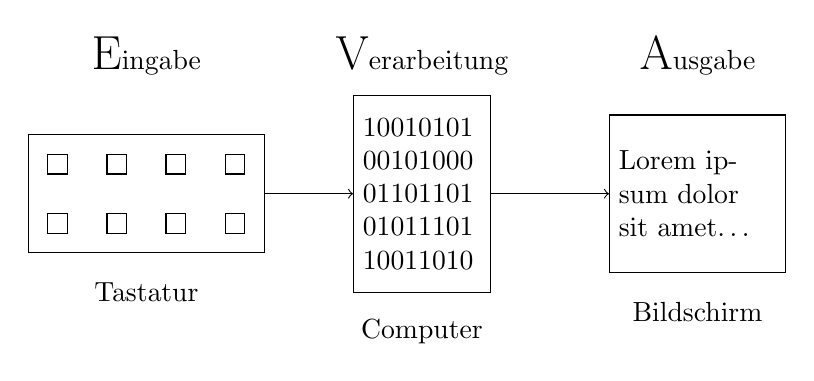
\begin{tikzpicture}[auto]
	\node[draw, rectangle, minimum width=3cm, minimum height=1.5cm] (start) at (1.5,0.75){};
	\node[below of=start, node distance = 1.25cm]{Tastatur};
	\foreach \x in {0.25, 1.00, 1.75, 2.50}
	{
		\foreach \y in{0.25, 1.00}
			\draw (\x,\y) rectangle (\x+0.25,\y+0.25);
	}
	\node[draw, rectangle, right of=start, minimum height=2.5cm, text width = 1.5cm, minimum width = 1.5cm, node distance = 3.5cm] (second) {10010101 00101000 01101101 01011101 10011010};
	\node[below of=second, node distance = 1.75cm]{Computer};
	\node[above of=second, node distance = 1.75cm](secondb){\LARGE{V}\normalsize{erarbeitung}};
	\node[left of=secondb, node distance = 3.5cm] {\LARGE{E}\normalsize{ingabe}};
	\node[right of=secondb, node distance = 3.5cm] {\LARGE{A}\normalsize{usgabe}};
	\node[draw, rectangle, right of=second, minimum height=2cm, text width = 2cm, minimum width = 2cm, node distance = 3.5cm] (third) {Lorem ipsum dolor sit amet\dots};
	\node[below of=third, node distance = 1.5cm]{Bildschirm};

	\draw[->] (start.east) -- (second.west);
	\draw[->] (second.east) -- (third.west);
\end{tikzpicture}
\end{figure}
\Img{GI(V)-17.03.2009-IMG1}

\begin{description}
\item[Ziel:] Formale Darstellung der Ein-/Ausgaben eines Computers
		\begin{itemize}[label=\Ra]
		\item Repr�sentation von Daten
		\end{itemize}
\end{description}

\begin{anmerkung}
Computerprogramme sind ebenfalls Daten.
\end{anmerkung}

\section{Alphabet}
\Mark{Section 2.1}
\begin{fdefinition}
Eine endliche Menge, die nicht leer ist, von \indexn[Symbol]{Symbolen} $\Sigma$ hei�t \indexn{Alphabet}\index{$\Sigma$ (Alphabet)}. Die Elemente von $\Sigma$ hei�en \indexn[Buchstabe]{Buchstaben} (\indexn{Zeichen}, Symbole). \qed
\Mark{Definition 2.1}
\end{fdefinition}

\begin{beispiel}
\mbox{}\par
\begin{itemize}
\item $\Sigma_{\text{RGB}}$ = \gklamm{\text{\underline{rot}}, \text{\underline{gr�n}}, \text{\underline{blau}}}
\item $\Sigma_{\text{Bool}}$ = \gklamm{0, 1} das Boole'sche Alphabet
\item $\Sigma_{\text{lat}}$ = \gklamm{a, b, c, \dots, z} das lateinische Alphabet
\item $\Sigma_{\text{Tastatur}}$ = \gklamm{A, B, \dots, Z, \text{\textvisiblespace}, <, >, (, ), \dots}
\item $\Sigma_{\text{m}}$ =  \gklamm{0, \dots, m -1} f�r $m \grgl 1$ die $m$-adische Darstellung einer Zahl.
\item $\Sigma_{\text{logic}}$ = \gklamm{0, 1, x, (, ), \oder, \und, \neg} ein Alphabet f�r logische Ausdr�cke
\end{itemize}
\end{beispiel}

\section{Wort}
\begin{fdefinition}[Wort]
Sei $\Sigma$ ein Alphabet. Ein \indexn[Wort]{Wort}\index{$\lambda$ (Wort)} �ber $\Sigma$ ist eine endliche (eventuell leere) Folge von Buchstaben. Das leere Wort $\epsilon$ (oder manchmal auch $\lambda$) ist die leere Buchstabenfolge. Die Menge aller W�rter �ber $\Sigma$ bezeichnen wir mit $\Sigma^*$. Ferner sei $\Sigma^+ = \Sigma^* - \gklamm{\epsilon}$. Fortan gehen wir davon aus, dass $\epsilon \notin \Sigma$ gilt. \qed
\Mark{Definition 2.2}
\end{fdefinition}

\begin{beispiel}
$\overbrace{(0, 1, 0, 1, 0, 1, 0)}^{\text{Z}}$ ist ein Wort �ber $\Sigma_{\text{Bool}}$, $\Sigma_{\text{Tastatur}}$ und $\Sigma_{\text{logic}}$.
\begin{itemize}
\item Z ist \underline{Wort} �ber $\Sigma_{\text{Bool}}$
\item Z ist aus $\Sigma_{Bool}^*$
\end{itemize}
$\epsilon$ ist ein Wort �ber einem \ac{bel.} Alphabet ($\epsilon \in \Sigma^*$ f�r alle Alphabete $\Sigma^*$)
\end{beispiel}

\begin{notation}
W�rter werden k�nftig ohne Kommata geschrieben und lassen auch die Klammern weg.\\
Also \ac{z.B.} 01010 statt (0,1,0,1,0)\\
Beachte: Unterschied Wort TI (Folge von Symbolen) und Wort \ggq{Deutsch}
\end{notation}

\subsection{Wortl�nge}
\begin{fdefinition}[Wortl�nge]
Sei $\Sigma$ ein Alphabet und $w \in \Sigma^*$. Die \indexn[Wort!Wortl�nge]{Wortl�nge} $\betrag{w}$ eines Wortes $w$ ist die L�nge des Wortes als Folge. F�r $a \in \Sigma$ bezeichnet $\betrag{w}_a$ die Anzahl der Vorkommen von $a$ in $w$. \qed
\Mark{Definition 2.3}
\end{fdefinition}

\begin{beispiel}
\mbox{}\par
\begin{itemize}
\item $\betrag{001001} = 6$
\item $\betrag{001001}_1 = 2$
\item $\betrag{\epsilon} = 0$
\item $\betrag{\text{\textvisiblespace}} = 1$
\end{itemize}
\end{beispiel}

\section{Konkatenation und Verkettung}
\begin{fdefinition}[Konkatenation/Verkettung]
Die \indexn[Alphabet!Konkatenation]{Konkatenation} f�r ein Alphabet $\Sigma$ ist eine Abbildung (oder auch Funktion) $K$:
\[\Sigma^* \times \Sigma^* \ra \Sigma^*\text{, so dass} K(u, v) = uv\]
f�r alle $u, v \in \Sigma^*$. Anstelle von $K(u, v)$ schreiben wir $u \mal v$. \qed
\Mark{Definition 2.4}
\end{fdefinition}

\begin{beobachtung}Konkatenation ist assoziativ. \Ra $(a \mal b) \mal c = a (b \mal c)$\\
Ferner gilt: $\epsilon \mal w = w = w \mal \epsilon$ Monoid.
\end{beobachtung}

\section{Induktive Definitionen}
\subsection{Induktive Definition des Wortbegriffes}
Die Menge aller W�rter �ber $\Sigma$ ($\Sigma^*$) ist induktiv definiert durch:
\begin{enumerate}
\item $\epsilon \in \Sigma^*$
\item sei $w \in \Sigma^*$ und $a \in \Sigma$, so $w \mal a \in \Sigma^*$\\
		\begin{center}
		\begin{tikzpicture}
			\node{}
			child[draw, rectangle]{
				child[draw, rectangle]{
					child[draw, rectangle]{
						child{node[draw, rectangle]{$\epsilon$}}
						child{node[draw, circle]{a}}}
					child{node[draw, circle]{b}}}
				child{node[draw, circle]{c}}};
		\end{tikzpicture}
		\end{center}
\end{enumerate}

\subsection{Induktive Definition der Wortl�nge}
\begin{enumerate}
\item f�r $w = \epsilon$ sei $\betrag{w} = 0$
\item f�r $w = v \mal x$ ist $\betrag{w} = \betrag{v} + 1$
		\begin{align*}
			\betrag{\underbrace{\epsilon a b}_{v} \underbrace{c}_{x}} &= \betrag{\underbrace{\epsilon a}_{v} \underbrace{b}_{x}} + 1\\
			&= \betrag{\underbrace{\epsilon}_{v} \underbrace{a}_{x}} + 1 + 1\\
			&= \betrag{\epsilon} + 1 + 1 + 1\\
			&= 0 + 1 + 1 + 1\\
			&= 3
		\end{align*}
\end{enumerate}

\section{Kanonische Ordnung}
\index{Kanonische Ordnung}
Um alle W�rter aus $\Sigma^*$ systematisch aufzuz�hlen, ordnen wir Alphabet und W�rter.
\begin{fdefinition}[Kanonische Ordnung]
Sei $\Sigma = \gklamm{a_1, a_2, \dots, a_n}$ und $<: \Sigma \times \Sigma$ eine Ordnung auf $\Sigma$ mit $a_1 < a_2 < a_3 < \dots < a_n$. Wir definieren die kanonische Ordnung auf $\Sigma^*$ wie folgt:
\[u < v \text{ \ac{gdw.} } \betrag{u} < \betrag{v} \oder\]
\[\betrag{u} = \betrag{v} \und u = w a_i u_1 \und v w a_j u_2 \text{ f�r } u, v \in \Sigma^* w, u_1, u_2 \in \Sigma^* \text{ und } a_i < a_j (i < j)\] \qed
\Mark{Definition 2.5}
\end{fdefinition}

\section{Teilwort, Pr�fixe, Suffixe}
\begin{fdefinition}[Teilwort, Pr�fixe, Suffixe]
Sei $\Sigma$ ein Alphabet und seien $v, w \in \Sigma^*$
\begin{itemize}
\item $v$ hei�t \indexn[Wort!Teilwort]{Teilwort} von $w$ \ac{gdw.} $\exists s, t \in \Sigma^*$: $w = s v t$
\item $v$ hei�t \indexn[Wort!Suffix]{Suffix} von $w$ \ac{gdw.} $\exists s \in \Sigma^*$: $w = sv$\\
		\begin{center}
		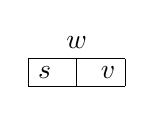
\begin{tikzpicture}
			\draw (0,0) -- (3.5em,0);
			\draw (3.5em,0) -- (3.5em,1em) node[left, midway]{$v$};
			\draw (3.5em,1em) -- (0,1em) node[above, midway]{$w$};
			\draw (0,1em) -- (0,0) node[right, midway]{$s$};
			\draw (1.75em,0) -- (1.75em,1em);
		\end{tikzpicture}
		\end{center}
		\Img{GI(V)-25.03.2009-IMG1}

\item $v$ hei�t \indexn[Wort!Pr�fix]{Pr�fix} von $w$ \ac{gdw.} $\exists t \in \Sigma^*$: $w = vt$\\
		\begin{center}
		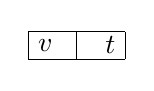
\begin{tikzpicture}
			\draw (0,0) -- (3.5em,0);
			\draw (3.5em,0) -- (3.5em,1em) node[left, midway]{$t$};
			\draw (3.5em,1em) -- (0,1em);
			\draw (0,1em) -- (0,0) node[right, midway]{$v$};
			\draw (1.75em,0) -- (1.75em,1em);
		\end{tikzpicture}
		\end{center}
		\Img{GI(V)-25-03.2009-IMG2}

\item $v \neq \epsilon$ hei�t \underline{echtes} Teilwort (Pr�fix/Suffix) von $w$ \ac{gdw.} $v \neq w$ und $v$ ist Teilwort (Pr�fix/Suffix) von $w$.
\end{itemize} \qed
\Mark{Definition 2.6}
\end{fdefinition}

\section{Wortumkehr}
\index{Wortumkehr}
\begin{fdefinition}[Wortumkehr]
Sei $\Sigma$ ein Alphabet und sei $w = a_1 \mal a_2 \mal a_3 \dots a_n$ mit $a_i \in \Sigma (1 \klgl i \klgl n)$ ein Wort. Dann ist die Wortumkehr $w^{\mathcal{R}}$ von $w$ \ac{def.} durch $w^{\mathcal{R}} = a_n a_{n - 1} \dots a_2 a_1$ \qed
\Mark{Definition 2.7}
\end{fdefinition}

\subsection{Alternativ: induktive Definition}
\begin{itemize}
\item $\epsilon^{\mathcal{R}} = \epsilon$
\item falls $v = w \mal a$, so $v^{\mathcal{R}} = a w^{\mathcal{R}}$
\end{itemize}

\begin{beispiel}
$(\overline{a}\overline{b}\overline{c})^{\mathcal{R}}$ $v = \overline{a}\overline{b}\overline{c}$ $w = \overline{a}\overline{b}$ $a = \overline{c}$
\begin{align*}
\Ra v^{\mathcal{R}} &= \overline{c} \mal \underbrace{(\overline{a}\overline{b})^{\mathcal{R}}} v = \overline{a}\overline{b} w = \overline{a} a = \overline{b}\\
\Ra v^{\mathcal{R}} &= \overline{c} \overline{b} \mal (\overline{a})^{\mathcal{R}} v = \epsilon \mal \overline{a} w = \epsilon a = \overline{a}\\
v^{\mathcal{R}} &= \overline{c} \mal \overline{b} \mal \overline{a} \mal (\epsilon)^{\mathcal{R}}\\
&= \overline{c} \mal \overline{b} \mal \overline{a} \mal \epsilon\\
&= \overline{c} \mal \overline{b} \mal \overline{a}
\end{align*}
\end{beispiel}

\section{Iteration}
\begin{fdefinition}[Iteration]
Sei $\Sigma$ ein Alphabet. F�r alle W�rter $w \in \Sigma^*$ und $i \in \mb{N}$ definieren wir die $i$-te Iteration $w^i$ als 
\[w^0 = \epsilon, w^1 = w\]
und
\[w^i = w \mal w^{i -1}\]
\Mark{Definition 2.8}
\end{fdefinition}

\begin{beispiel}
\begin{align*}
aabb \mal bbab &= aabbbbab\\
&= a^2 b^4 ab\\
ababc &= (ab)^2 c
\end{align*}
\end{beispiel}

\section{Sprachen}
\index{Sprache}
\index{Sprache!Konkatenation}
\index{Kleene-Stern}
\index{$L$ (Sprache)}
\begin{fdefinition}[Sprache, Konkatenation von Sprachen, Kleene-Stern]
Sei $\Sigma$ ein Alphabet. Eine \indexn{Sprache} $L$ ist eine Teilmenge von $\Sigma^*$ ($L \subseteq \Sigma^*$) (potentiell unendlich!). Das \indexb[Sprache!Komplement]{Komplement}\index{\space^{\mathcal{C}} (Komplement)} $L^{\mathcal{C}}$ der Sprache $L$ bez�glich $\Sigma^*$ ist die Sprache $\Sigma^* - L$. $L_{\emptyset}$ ist die leere Sprache; $L_{\epsilon} = \gklamm{\epsilon}$. Seien $L_1$ und $L_2$ Sprachen, dann ist
\[L_1 \mal L_2 = L_1 L_2 = \gklamm{u \mal v \in \left(\Sigma_1 \cup \Sigma_2\right)^x \vert u \in L_1 \und v \in L_2}\]
die Konkatenation von $L_1$ und $L_2$. Ferner definieren wir f�r eine Sprache $L$
\[L^0 = L_{\epsilon} L^{i + 1} = L \mal L^i\]
und
\[L^* = \bigcup_{i \in \mb{N}} L^i \text{ und } L^+ = \bigcup_{i \in \mb{N} - \gklamm{0}} L^i = L \mal L^*\]
\Mark{Definition 2.9}
\end{fdefinition}

\begin{beispiel}
\mbox{}\par
\begin{multicols}{2}
\begin{itemize}
\item $L_1 = \emptyset$
\item $L_2 = \gklamm{\epsilon}$
\item $L_3 = \gklamm{\epsilon, aa, bb, ab, ba}$
\item $L_4 = \gklamm{a, b}^* = \{\epsilon, a, b, aa,$\\
	  $ab, ba, bb, \dots\}$

\item $L_5 = \gklamm{a}^* = \gklamm{\epsilon, a, aa, aaa, \dots} = \gklamm{a^0, a^1, a^2, \dots}$
\item $L_6 = \gklamm{a^p \vert p = \text{ Primzahl}}$
\item $L_7 = \gklamm{a^i b^{2i} a^i \vert i \in \mb{N}}$
\item $L_8 =$ alle syntaktisch korrekten \textit{JAVA}-Programme.
\item $L_9 =$ alle typ-korrekter \textit{JAVA}-Programme.
\item $L_{10} =$ alle terminierenden \textit{JAVA}-Programme.
\end{itemize}
\end{multicols}
\end{beispiel}

\begin{enumerate}
\item Sprachen geeignet zur Darstellung aller Ein/Ausgaben?
\item Reicht $\Sigma_{\text{Bool}}$?
\item Effizienter Test, ob $w \in L$ gilt. \fbox{\la Automaten}
\item Wie kann man Sprachen formal definieren? \fbox{\la Grammatiken}
\item Sind Sprachen aufz�hlbar? \fbox{\la Berechenbarkeit}\\
		Effizient m�glich. \fbox{\la Komplexit�tstheorie}
\end{enumerate}

\begin{lemma}
Seien $L_1$, $L_2$ und $L_3$ Sprachen �ber einem Alphabet $\Sigma$. Dann gilt
\[L_1 \mal L_2 \cup L_1 \mal L_3 = L_1 \mal (L_2 \cup L_3)\]
\end{lemma}

\begin{fbeweis}
\mbox{}\par
\begin{itemize}
\item $L_1 \mal L_2 \cup L_1 \mal L_3 \subseteq L_1 \mal (L_2 \cup L_3)$
		\begin{itemize}
		\item $L_1 \mal L_2 \subseteq L_1 \mal (L_2 \cup L_3)$
				\begin{align*}
				L_1 \mal L_2 &= \gklamm{uv \vert u \in L_1 \und v \in L_2}\\
				&\subseteq \gklamm{uv \vert u \in L_1 \und L_2 \cup L_3}\\
				&= L_1 \mal (L_2 \cup L_3)
				\end{align*}
		\item $L_1 \mal L_3 \subseteq L_1 \mal (L_2 \cup L_3)$\\
				\ra analog
		\end{itemize}

\item $L_1 \mal (L_2 \cup L_3) \subseteq L_1 \mal L_2 \cup L_1 \mal L_3$
		\begin{align*}
		&x \in L_1 \mal (L_2 \cup L_3) \text{ beliebig}\\
		\Lra & x \in \gklamm{uv \vert u \in L_1 \und v \in L_2 \cup L_3} \text{ (Definition Konkatenation)}\\
		\Lra & \exists u \in L_1 \und \exists v \in L_2 \cup L_3: x = uv \text{ (�bergang zur Pr�dikaten Logik)}\\
		\Lra & \exists u \in L_1 \und (\exists v \in L_2 \oder \exists v \in L_3): x = uv \text{ (�bergang Pr�dikaten Logik 2)}\\
		\Lra & (\exists u \in L_1 \und \exists v \in L_2: x = uv) \oder (\exists u \in L_1 \und \exists v \in L_3: x = uv)\\ &\text{(Distributivgesetz der Pr�dikaten Logik)}\\
		\Lra & x \in \underbrace{\gklamm{uv \vert u \in L_1 \und v \in L_2}}_{= L_1 \mal L_2} \oder x \in \underbrace{\gklamm{uv \vert u \in L_1 \und v \in L_3}}_{= L_1 \mal L_3}\\
		\Lra & x \in L_1 \mal L_2 \oder x \in L_1 \mal L_3\\
		\Lra & x \in L_1 \mal L_2 \cup L_1 \mal L_3
		\end{align*}
\end{itemize}
\end{fbeweis}

\section{Sprachen zur Beschreibung von Problemen}
\Mark{Section 2.3}
\subsection{Entscheidungsprobleme}
\Mark{Subsection 2.3.1}
\begin{fdefinition}
Das Entscheidungsproblem ($\Sigma$, $L$) f�r ein gegebenes Alphabet $\Sigma$ und eine Sprache $L \in \Sigma^*$ ist, f�r jedes $w \in \Sigma^*$ zu entscheiden, ob
\[w \in L \oder w \notin L\]
\[\Sigma_{\text{Input}}^* \longrightarrow \fbox{$\Sigma_{\text{Bool}}^* \ra \Sigma_{\text{Bool}}^*$} \longrightarrow \Sigma_{\text{Output}}^*\]
\end{fdefinition}

Ein Algorithmus l�st das Entscheidungsproblem ($\Sigma$, $L$), falls $\forall w \in \Sigma^*$
\[A(w) = \begin{cases}1 & w \in L\\0 & \text{sonst.}\end{cases}\]
Wir sagen auch, dass $A$ $L$ erkennt.

\begin{fdefinition}
Existiert f�r eine Sprache $L$ ein Algorithmus, der diese erkennt, so hei�t $L$ \underline{rekursiv}.
\end{fdefinition}

\begin{beispiel}
Ein wichtiges Entscheidungsproblem ist der Primzahltest.
\[\rklamm{\Sigma_{\text{Bool}}, \gklamm{w \in \Sigma_{\text{Bool}}^* \vert \text{Zahlwert }(w)\text{ ist Primzahl}}}\]
\end{beispiel}

\begin{beispiel}
Das Erf�llbarkeitsproblem.
\[\rklamm{\Sigma_{\text{logic}}m \gklamm{w \in \Sigma_{\text{logic}}^* \vert w \text{ erf�llbar}}}\]
\[\neg \rklamm{A_1 \oder A_2} \und A_3 \und A_4 \und \neg A_4\]
Ein ebenfalls wichtiges Entscheidungsproblem ist die Frage der �quivalenz von Algorithmen $A$ und $B$.
\[\rklamm{\Sigma_{\tx{Tastatur}}, \gklamm{B \vert B \tx{ ist �quivalent zu } A}}\]
$A$ ist �quivalent zu $B$, falls $A$ auf jede m�gliche Eingabe genauso reagiert wie $B$ und umgekehrt $A$.
\[\fbox{A} \stack{\text{Optimiert}}{\longrightarrow} \fbox{B}\]
\end{beispiel}

\subsection{\texorpdfstring{Aufz�hlungsalgorithmus f�r $L$}{Aufz�hlungsalgorithmus f�r L}}
\begin{fdefinition}
Sei $\Sigma$ ein Alphabet und $L \subseteq \Sigma^*$. $A$ ist ein Aufz�hlungsalgorithmus f�r $L$, falls $A$ f�r jede Eingabe $n \in \mb{N} - \rklamm{0}$ die kanonisch (siehe Kanonische Ordnung) ersten $n$ W�rter $w_0, w_1, \dots w_{n -1}$ der Sprache $L$ ausgibt.
\end{fdefinition}

\begin{lemma}
Sei $\Sigma$ ein Alphabet und $L \subseteq \Sigma^*$.
\begin{itemize}
\item $L$ ist rekursiv $\stackrel{\tx{\ac{gdw.}}}{\Lra}$ es existiert Aufz�hlungsalgorithmus f�r $L$
\item $L$ entscheidbar
\end{itemize}
\end{lemma}

\subsection{Funktionsberechnungen}
\begin{fdefinition}[Funktionsproblems]
Seien $\Sigma_D$ und $\Sigma_W$ zwei Alphabete. Wir sagen, dass ein Algorithmus $A$ eine Funktion $f: \Sigma_D^* \ra \Sigma_W^*$ berechnet (oder das Funktionsproblem $f$ l�st), falls
\[\forall w \in \Sigma_D^*: A(w) = f(w)\]
Existiert ein Algorithmus, der $f$ berechnet, so hei�t $f$ berechenbar.
\end{fdefinition}

\subsection{Relationsprobleme}
\begin{fdefinition}
Seien $\Sigma_1$ und $\Sigma_2$ Alphabete und $R \subseteq \Sigma_1^* \times \Sigma_2^*$ eine Relation. Ein Algorithmus $A$ berechnet $R$ (oder l�st das Relationsproblem $R$), falls f�r jedes $w \in \Sigma_1^*$ gilt:
\[\rklamm{w, A(w)} \in R\]
\end{fdefinition}

\section{Kolmogorov Komplexit�t}
\Mark{Section 2.4}
\begin{beispiel}[Wortl�nge vs. Informationsgehalt]
Das Wort
\[w = 01 01 01 01 01 01 01\]
ist zwar l�nger als das Wort
\[v = 10 10 11 00\]
kann aber durch $(01)^7$ kompakter dargestellt werden. Es reichen offenbar f�nf Zeichen um die Information in $w$ zu kodieren.
\end{beispiel}

Das Auffinden einer k�rzeren Darstellung f�r ein Wort nennt man \indexb{Komprimierung}.
\begin{description}
\item[Ziel:] Um den Informationsgehalt zweier W�rter zu vergleichen, k�nnten
wir zun�chst ein Standard Komprimierungs Verfahren suchen.\\
\item[Problem:] Wie findet man ein Verfahren, welches immer die kleinstm�gliche Darstellung garantiert?
\end{description}

\begin{beispiel}[Laufl�ngenkodierung]
Wir �berf�hren eine Bin�rzahl zun�chst in die Darstellung
\[b_1^{l_1} b_2^{l_2}\dots, b_i \in \Sigma_{\tx{Bool}}^*\]
wobei wir auch die Exponenten in Bin�rschreibweise darstellen. Von dieser Darstellung gehen wir wie folgt �ber zu einem Wort �ber $\Sigma_{\sharp} = \rklamm{0, 1, \sharp}$
\[l_1 \sharp b_1 \sharp l_2 \sharp b_2 \dots\]
Nach $\Sigma_{\tx{Bool}}$ kommen wir durch Anwendung eines Homomorphismus.\\
$\Sigma = \gklamm{0, 1, \sharp}$
\[\left.\begin{array}{l}
h (0) = 00\\
h (1) = 11\\
h (\sharp) = 10
\end{array} \right\} h: \Sigma_{\sharp} \ra \Sigma_{\tx{Bool}}^*\]
\[h (a_1 \dots a_n) = h(a_1) \mal h(a_2) \mal \dots \mal h(a_n)\]
\[k (00\sharp 1) = \begin{array}{ccccccc}
h(0) & \mal & h(0) & \mal & h(\sharp) & \mal & h(1)\\
00 && 00 && 01 && 11\\
0 && 0 && 10 && 1
\end{array}\]
$H: \Sigma_1^* \ra \Sigma_2^*$
\begin{itemize}
\item $h(\epsilon) = \epsilon$
\item $h(u \mal v) = h(u) \mal h(v)$
\end{itemize}
\end{beispiel}

\begin{beispiel}
Sei $w = (100)^{11} (101)^3 (01)^3 \betrag{w} = 43$\\
In unserer Zwischendarstellung ist dies
\[1011\sharp 100\sharp 11\sharp 101\sharp 11\sharp 01\sharp\]
und mit dem Homomorphismus $h(0) = 00$, $h(1) = 11$ und $h(\sharp) = 10$ gelangen wir zu
\[11 00\, 11 11\, 10 11\, 00 00\, 10 11\, 11 10 \dots \text{ mit } \betrag{w'} = 42\]
\end{beispiel}

F�r gro�e Exponenten kann es sich lohnen, die Laufl�ngenkodierung auch auf diese Anzuwenden. Zum Beispiel:
\[(011)^{1048576} = (011)^{2^{20}}\]

Diese Strategie kann man beliebig fortsetzen, um zum Beispiel W�rter der Bauarten $(01)^{2^{2^n}}$ oder $(01)^{2^{2^{2^n}}}$ zu kodieren.\\
Allgemeines kompressions Verfahren wird durch anderen Umstand ebenfalls schwer auffindbar.

\begin{beispiel}[Codierung durch Primfaktorzerlegung]
Jede Zahl k�nnen wir als Folge von Primfaktoren eindeutig darstellen: zum Beispiel $884736 = 2^1 \mal 3^3 \mal 4^7$. Unter Einbeziehung der Basis k�nnen wir dies darstellen als.
\[\bin(e_1) \sharp \bin(p_1) \sharp \bin(e_2) \sharp \dots\]
Verfahren der Primfaktorzerlegung und der Laufl�ngenkodierung sind \textbf{unvergleichbar}. Eines der beiden Verfahren ist Grunds�tzlich besser.
\end{beispiel}

\begin{fdefinition}
F�r alle W�rter $w \in \Sigma_{\tx{Bool}}^*$ ist die Kolmogorov-Komplexit�t $K_c(w)$ definiert als die bin�re L�nge \textit{des k�rzesten \lstinline{C++} Programmes}, welches $w$ generiert.
\end{fdefinition}

\begin{lemma}
Es existiert eine Konstante $d$, so dass f�r jedes $w \in \Sigma_{\tx{Bool}}^*$ gilt:
\[K_c (w) \klgl \betrag{w} + d\]
\end{lemma}

\begin{fbeweis}
F�r jedes $w$ aus $\Sigma_{\tx{Bool}}^*$ nehmen wir folgendes \lstinline{C++} Programm:
\[P(\underbrace{w}_{\tx{Zeichenkette}}) = \left\{
\begin{minipage}{82mm}
\begin{lstlisting}[language=C++]
int main(int args, char** args) {
	char * ws = w; //"abcdefg"
	count++ w;
}
\end{lstlisting}
\end{minipage}\right.\]
\end{fbeweis}

Regelm��ige W�rter haben eine geringere Kolmogorov-Komplexit�t. Betrachte \ac{z.B.} W�rter der Bauart $v_n = 0^n$ f�r $n \in \mb{N} \backslash \gklamm{0}$
\[P(n) = \left\{
\begin{minipage}{70mm}
\begin{lstlisting}[language=C++]
unsigned int n;
for(int i = 1; i <= n; i++)
	cout << "0";
\end{lstlisting}
\end{minipage}\right.\]
Bis auf die konstante $n$ sind alle $P(n)$ identisch. Zur Kodierung von $n$ als Bin�rzahl ben�tigt man $\lceil \ld (n + 1)\rceil$ Bits. Damit
\[K_c (v_n) \klgl \lceil \ld (n + 1) \rceil + c \klgl \lceil \ld n \rceil + c' = \lceil \ld \betrag{v_n} \rceil + c'\]

Betrachte $u_n = 0^{n^2}$ $n \in \mb{N} - \gklamm{0}$
\[P(n) \begin{cases}
\begin{minipage}{2.5cm}
\begin{center}
$\cancel{\mbox{\lstinline!m = n + n!}}$
\end{center}
\end{minipage}
\left|
\begin{minipage}{65mm}
\begin{lstlisting}
m = n;
m = m * m;
for(int i = 1; i <= m; i++)
	cout << "0";
\end{lstlisting}
\end{minipage}\right.
\end{cases}\]
\[K_c (u_n) \klgl \lceil \ld n \rceil + c \klgl \lceil \ld \sqrt{\betrag{u_n}} \rceil + c\]
\begin{align*}
&\betrag{u_n} = n^2\\
\Lra &n = \sqrt{\betrag{u_n}}
\end{align*}

\begin{fdefinition}
Sei $n \in \mb{N}$. Die Kolmogorov-Komplexit�t
\[K_c (n) = K_c(\bin(n))\tx{.}\]
\end{fdefinition}

\begin{lemma}
F�r jedes $n \in \mb{N} \backslash {0}$ existiert ein Wort $w_n \in \Sigma_{Bool}^n$, so dass
\[K_c (w_n) \grgl \betrag{w_n}\]
\textbf{Es gibt W�rter der L�nge $n$, die nicht komprimierbar sind.}
\end{lemma}

\begin{fbeweis}
Wir haben genau $2^n$ W�rter $x_1, \dots, x_{2^n} \in \Sigma_{\tx{Bool}}^n$. Sei f�r $i = 1, \dots, 2^n \prog(x_i)$ der Maschinencode des \lstinline{C++} Programmes von $x_i$ und sei $K_c (x_i) = \betrag{\prog(x_i)}$ die L�nge eines k�rzesten Algorithmus. Es ist klar, dass f�r $x_i \neq x_j$ gilt: 
\[\prog(x_i) \neq \prog(x_j)\]
wir haben also $2^n$ unterschiedliche Programme. Es gen�gt zu zeigen, dass eines dieser Programme die L�nge $n$ hat.

Jetzt hilft das kombinatorische Argument: es ist unm�glich $2^n$ verschiedene Maschinencodes der L�nge kleiner als $n$ zu haben, denn die Anzahl aller unterschiedlichen, nicht leeren, W�rter aus $\Sigma_{\tx{Bool}}^{n - 1}$ ist
\[\sum_{i = 1}^{n - 1} 2^i = 2^n - 2 < 2^n\]
Also muss es unter den $2^n$ Programmen mindestens eins der L�nge $n$ geben.
\end{fbeweis}

\begin{fsatz}
Seien $A$ und $B$ Programmiersprachen. Es existiert eine Konstante $c_{A, B}$, die nur von $A$ und $B$ abh�ngig ist, so dass $\forall w \in \Sigma_{\tx{Bool}}^*$
\[\betrag{K_{c_A} (w) - K_{C_B}} \klgl c_{A, B}\]
\end{fsatz}

\begin{fbeweis}
trivial
\end{fbeweis}

\begin{fdefinition}[Zuf�llig]
Ein Wort $w \in \Sigma_{\tx{Bool}}^*$ hei�t zuf�llig, falls $K_C (w) \grgl \betrag{w}$. Eine Zahl $n$ hei�t zuf�llig, falls
\[K_c(n) = K_c (\bin(n)) \grgl \lceil \ld(n + 1) \rceil - 1\]
\end{fdefinition}

%\chapter{Endliche Automaten}
\Mark{Kapitel 3}
\begin{fdefinition}[\ac{DEA}]
Ein \ac{DEA} ist ein Quintupel $M = (Q, \Sigma, \delta, q_0, F)$ aus
\begin{itemize}
\item einer endlichen Menge von Zust�nden $Q$
\item einem Eingabealphabet $\Sigma$
\item einer Transitionsfunktion $\delta$: $Q \times \Sigma \ra Q$
\item einen Startzustand $q_0 \in Q$
\item eine Menge von akzeptierenden Zust�nden $F \subseteq Q$\\
		\begin{anmerkung}
		$F$ kann leeres Element sein also kann der Automat auch keine Zust�nde annehmen!
		\end{anmerkung}
\end{itemize}
\Mark{Definition 3.1}
\end{fdefinition}

\begin{fnotation}
Anstelle von $\delta(q, a) = q$ schreiben wir
\[p \stack{a}{\longrightarrow}_M q\]
\end{fnotation}

\begin{beispiel}
\mbox{}\par
\Img{GI(V)-15.04.2009-DIA-1}
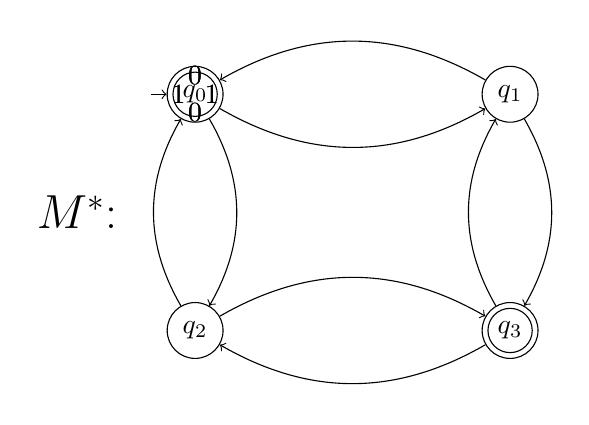
\begin{tikzpicture}[node distance = 3cm]
\node at(-1.5cm,-1.5cm) {\LARGE{$M^*$:}};

\node[circle,draw] (q0) {$q_0$};
\node[circle,draw] (q1) [right of=q0, node distance = 4cm] {$q_1$};
\node[circle,draw] (q2) [below of=q0] {$q_2$};
\node[circle,draw] (q3) [below of=q1] {$q_3$};

\draw[->] (q0.west) +(-0.2,0) -- (q0.west);

\draw[<-] (q0) to [out=30,in=150] (q1) node[above, midway] {$0$};
\draw[->] (q0) to [out=-30,in=-150] (q1) node[below, midway] {$0$};
\draw[->] (q2) to [out=30,in=150] (q3) node[above, midway] {$0$};
\draw[<-] (q2) to [out=-30,in=-150] (q3) node[below, midway] {$0$};

\draw[->] (q0) to [out=-60,in=60] (q2) node[right, midway] {$1$};
\draw[<-] (q0) to [out=-120,in=120] (q2) node[left, midway] {$1$};

\draw[->] (q1) to [out=-60,in=60] (q3) node[right, midway] {$1$};
\draw[<-] (q1) to [out=-120,in=120] (q3) node[left, midway] {$1$};

\draw (q0.center) circle (8pt);
\draw (q3.center) circle (8pt);
\end{tikzpicture}

$M = \rklamm{\gklamm{q_0, q_1, q_2, q_3}, \Sigma_{\tx{Bool}}m, \delta, q_0, \gklamm{q_0, q_3}}$ mit $\delta$:
\begin{table}[htb]
\begin{tabular}{c|c|c}
& $0$ & $1$\\\hline
$q_0$ & $q_1$ & $q_2$\\
$q_1$ & $q_0$ & $q_3$\\
$q_2$ & $q_3$ & $q_0$\\
$q_3$ & $q_2$ & $q_1$
\end{tabular}
\end{table}
\end{beispiel}

\begin{fdefinition}
Sei $M = (Q, \Sigma, \delta, q_0, F)$ ein \ac{DEA}. Eine \indexn{Konfiguration} von $M$ ist ein Paar aus $Q \times \Sigma^*$. $(q_0, w)$ hei�t \indexn{Startkonfiguration} und $(q, \epsilon)$ \indexn{Endkonfiguration} (f�r \ac{bel.} $w \in \Sigma^*$). Gilt f�r eine Endkonfiguration $(q, \epsilon)$ das $q \in F$, so hei�t diese akzeptierend, ansonsten verwerfend. \qed
\Mark{Definition 3.2}
\end{fdefinition}

\begin{fdefinition}
Sei $M = (Q, \Sigma, \delta, q_0, F)$ ein \ac{DEA}. Ein \indexn{Konfigurations�bergang} (ein Schritt) ist eine Relation $\vd_M$: $(Q \times \Sigma^*) \times (Q \times \Sigma^*)$, die \ac{def.} ist durch
\[(p, \underbrace{a}_{\tx{Lesekopf}}\overbrace{w}^{\tx{Band}}) \vd (q, w) \tx{ \ac{gdw.} } \delta(p, a) = q\]

\begin{center}
    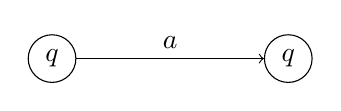
\begin{tikzpicture}[node distance = 3cm]
\node[circle,draw] (nodeone) {$q$};
\node[circle,draw] (nodetwo) [right of=nodeone] {$q$};

\draw[->] (nodeone.east) -- (nodetwo.west) node[above, midway] {$a$};
\end{tikzpicture}
\end{center}

mit $p, q \in Q$, $w \in \Sigma^*$ und $a \in \Sigma$. $\vd_u$ nennen wir \indexn{Schrittrelation}.
\Mark{Definition 3.3}
\end{fdefinition}

\begin{fdefinition}
Sei $M = (Q, \Sigma, \delta, q_0, F)$ ein \ac{DEA} und $w \in \Sigma^*$. Eine Berechnung $c$ von $M$ ist eine endliche Folge von Konfigurationen
\[c = c_0, \dots, c_n \tx{ mit } c_i \vd c_{i + 1} (1 \klgl i \klgl n - 1)\]
$c$ ist eine Berechnung von $M$ f�r eine Eingabe $w$, falls $c_0 = (q_0, w)$ (Startkonfiguration) und $c_n = (q, \epsilon)$ (Endkonfiguration). Falls $c_n$ \ac{akzept.} Endkonfiguration ist, so ist C \ac{akzept.} Berechnung; ansonsten verwerfende Berechnung.
\Mark{Definition 3.4}
\end{fdefinition}

\begin{beispiel}
\[(q_0, \underline{1}001) \vd (q_2, 001) \vd (q_3, 01) \vd (q_2, 1) \vd (\underbrace{q_0}_{\in F}, \epsilon)\]
ist \ac{akzept.} Berechnung von $M^*$ (zu GI(V)-15.04.2009-DIA-1) auf $1001$
\end{beispiel}

\begin{fdefinition}
Sei $M = (Q, \Sigma, \delta, q_0, F)$ ein \ac{DEA}. Wir definieren: $\vd_M^*$: $(Q \times \Sigma^*) \times (Q \times \Sigma^*)$ als reflexiven und transitiven Abschluss von $\vd$:
\begin{itemize}
\item $(q, w) \vd^* (q, w)$ $\forall q \in Q, w \in \Sigma^*$
\item $(p, uv) \vd^* (q, v)$, falls $u = a_1 \dots a_n (a_i \in \Sigma)$ $\exists q_1, \dots, q_{n - 1} \in Q$, so dass
		\[(p, a_1 \dots a_n v) \vd (q_1, a_1 \dots a_n v) \vd \dots \vd (q_{n - 1}, a_n v) \vd (q, v)\]
		f�r $p, q \in Q$ $u, v \in \Sigma^*$
\end{itemize}
Die Fortsetzung $\hat{\delta}$: $Q \times \Sigma^* \ra Q$ der Transitionsfunktion $\delta$ auf W�rter \ac{def.} wir induktiv durch
\begin{itemize}
\item $\hat{\delta} (q, \epsilon) = q$
\item $\hat{\delta} (q, wa) = \delta(\hat{\delta} (q, w))$ $\forall w \in \Sigma^*$, $a \in \Sigma$ und $q \in Q$
\end{itemize}
\Mark{Definition 3.5}
\end{fdefinition}

\begin{fnotation}
Falls $\hat{\delta} (q, w) = p$, so schreiben wir
\[q \stack{w}{\longrightarrow} p\]
und sagen es existiert ein Pfad von $q$ nach $p$ mit Beschriftung $w$.
\end{fnotation}

\begin{fdefinition}
Sei $M = (Q, \Sigma, \delta, q_0, F)$ ein \ac{DEA}. Die von $M$ akzeptierte Sprache $L(M)$ ergibt sich aus:
\begin{align*}
L(M) &= \gklamm{w \in \Sigma^* \vert \hat{\delta}(q_0, w) \in F}\\
&= \gklamm{w \in \Sigma^* \vert q_0 \stack{w}{\longrightarrow} q \tx{ und } q \in F}\\
&= \gklamm{w \in \Sigma^* \vert (q_0, w) \vd^* (q, \epsilon) \tx{ mit } q \in F}
\end{align*}
Sprachen, die von einem \ac{DEA} erkannt werden nennt man regul�re Sprachen. Zwei \ac{DEA}s $M_1$ und $M_2$ sind �quivalent \ac{gdw.} $L(M_1) = L(M_2)$
\Mark{Definition 3.6}
\end{fdefinition}

\begin{lemma}
Der \ac{DEA} $M_x = \rklamm{\Sigma_{\tx{Bool}}, Q, \delta, q_0, F}$ erkennt die Sprache
\[L(M_x) = \gklamm{w \in \Sigma_{\tx{Bool}}^* \vert \rklamm{\betrag{w}_0 + \betrag{w}_1} \mod 2 = 0}\]
\end{lemma}

\begin{fbeweis}
F�r jedes Wort $w \in \Sigma_{\tx{Bool}}^*$ bleibt der Automat $M_x$ in einem bestimmten Zustand stehen. Betrachten wir f�r einen \ac{bel.} Zustand die Menge der W�rter, f�r die $M_x$ in exakt diesem Zustand terminiert.
\[\mathcal{K} (q) = \gklamm{w \in \Sigma_{\tx{Bool}}^*\vert q_0 \stack{w}{\longrightarrow} q}\]
Da $M_x$ deterministisch ist, kann ein Wort, welches in $\mathcal{K}(q)$ liegt nicht gleichzeitig in $\mathcal{K}\rklamm{q^{\frownie}}$ liegen (mit $q \neq q^{\frownie}$) - $\mathcal{K}(q) \cap \mathcal{K}\rklamm{q^{\frownie}} = \emptyset$. Die Menge der von $M_x$ erkannten W�rter entspricht der Vereinigung aller Mengen $\mathcal{K}(q)$, die sich auf akzeptierende Zust�nde beziehen.
\[L(M_x) = \bigcup_{q \in F} \mathcal{K}(q)\]
$\mathcal{K}$ ist eine �quivalenzklasse folgender Relation $R_s$
\begin{align*}
&u R_{\delta} v = \hat{\delta} (q_0, u) = \hat{\delta} (q_0, u)\\
&R_{\delta} (w, v)
\end{align*}
in $\mathcal{K} (q)$ befindet sich nur solche W�rter, die \ac{bzgl.} $R_{\delta}$ in Relation stehen.

Beweisidee:
\begin{itemize}[label=-]
\item Ordne $q_i (0 \klgl i \klgl 3)$ konkrete �quivalenz-Klassen zu \textcircled{$\star$}
\item Zeige $\mathcal{K} (q_0) \cup \mathcal{K} (q_3) = L(u)$
\item Zeige, dass \textcircled{$\star$} korrekt.
\end{itemize}
\Solved{�ndere \textcircled{*} in ein sch�neres Symbol}{Replaced with \textcircled{$\star$}}
Wir stellen folgende Induktionsannahme auf:
\begin{align*}
&\mathcal{K} (q_0) = \gklamm{w \in \Sigma_{\tx{Bool}}^*~\vert~\betrag{w}_0 \tx{ und } \betrag{w}_1 \tx{ sind gerade}}\\
&\mathcal{K} (q_1) = \gklamm{w \in \Sigma_{\tx{Bool}}^*~\vert~\betrag{w}_0 \tx{ ungerade } \vert \betrag{w}_1 \tx{ gerade}}\\
&\mathcal{K} (q_2) = \gklamm{w \in \Sigma_{\tx{Bool}}^*~\vert~\betrag{w}_0 \tx{ gerade } \vert \betrag{w}_1 \tx{ ungerade}}\\
&\mathcal{K} (q_3) = \gklamm{w \in \Sigma_{\tx{Bool}}^*~\vert~\betrag{w}_0 \tx{ und } \betrag{w}_1 \tx{ ungerade}}
\end{align*}

\begin{enumerate}
\item Induktionsanfang: wir zeigen, dass $\vert A$ f�r W�rter der L�nge $\klgl 2$ gilt
		\begin{align*}
		0:~~&\delta \rklamm{q_0, \epsilon} = q_0 \Ra \epsilon \in \mathcal{K}(q_0) \checkmark\\
		1:~~&\delta (q_0, 1) = q_2, 1 \in \mathcal{K}(q_2) \checkmark\\
			&\delta (q_0, 0) = q_1, 0 \in \mathcal{K}(q_1) \checkmark\\
		2:~~&\hat{\delta} (q_0, 00) = q_0, 00 \in \mathcal{K} (q_0) \checkmark\\
			&\hat{\delta} (q_0, 01) = q_3, 01 \in \mathcal{K} (q_3) \checkmark\\
			&\hat{\delta} (q_0, 10) = q_3, 10 \in \mathcal{K} (q_3) \checkmark\\
			&\hat{\delta} (q_0, 11) = q_0, 11 \in \mathcal{K} (q_0) \checkmark
		\end{align*}
\item Induktionsschluss: Wir setzen voraus, dass der Induktionsanfang f�r W�rter $\betrag{u} \klgl i$ gilt. Wir wollen jetzt zeigen, dass der Induktionsanfang dann auch f�r W�rter der L�nge $i + 1$ gilt.\\
		Sei also $w \in \Sigma_{\tx{Bool}}^{i + 1}$, also $w = u \mal a$ mit $u \in \Sigma_{\tx{Bool}}^{i}$ und $a \in \Sigma_{\tx{Bool}}$. Wir m�ssen vier F�lle unterscheiden:
		\begin{enumerate}[label=\arabic*.]
		\item $\betrag{u}_0$ gerade, $\betrag{u}_1$ gerade. Laut Induktionsvoraussetzung gilt $\hat{\delta} (q_0, u) = q_0$ \ac{bzw.} $u \in \mathcal{K} (q_0)$. Wir erhalten
				\[\hat{\delta} (q_0, ua) = \delta \rklamm{\hat{\delta} (q_0, u), a} \stack{\tx{IV}}{=} \delta(q_0, a) = \begin{cases}q_1 \tx{ falls } a = 0\\q_2 \tx{ falls } a = 1\end{cases}\]
				Da $\betrag{u1}_0$ gerade und $\betrag{u1}_1$ ungerade entspricht $\hat{\delta} (q_0, u1) = q_2$ der IA.\\
				Da $\betrag{u0}_0$ ungerade und $\betrag{u0}_1$ gerade entspricht $\hat{\delta} (q_0, u0) = q_1$ der IA.
		\item analog, trivial, selbst! 
		\item analog, trivial, selbst!
		\item analog, trivial, selbst!
		\end{enumerate}
\end{enumerate}
\end{fbeweis}

\section{Nichtdeterministische endliche Automaten (NEAs)}
\Mark{Section 3.3}
\Insert{IMG-GI-09-04-21-1}
\begin{fdefinition}
Ein \ac{NEA} $M$ ist ein Quintupel $(Q, \Sigma, \delta, q_0, F)$ aus
\begin{itemize}
\item $Q, \Sigma, q_0, F$ wie \ac{DEA}
\item eine Transitionsfunktion $\delta$: $Q \times \Sigma \ra \mathcal{P} (Q)$
\end{itemize}
\end{fdefinition}

\begin{fnotation}
Falls $q \in \delta(p, a)$ schreiben wir $p \stack{a}{\ra} q$
\end{fnotation}

\section{Anwendungen f�r Rabin-Scott-Automaten}
\Mark{Section 3.8}
\subsection{Textsuche}
\Mark{Subsection 3.8.1}
\Ra siehe AD (Knuth-Morris-Pralt Algorithmus)

\subsection{Analyse von Programmen}
\Mark{Subsection 3.8.2}
\begin{lstlisting}[language=C++]
x << cin;
a = x; /* a.1 */
b = x; /* b.1 */
while (p(a))
	a = f(a); /* a.2 */
while (q(b)){
	a = g(a); /* a.3 */
	b = f(b); /* b.2 */
}
z = a; /* z.1 */
cout << z;
\end{lstlisting}
\begin{frage}
was berechnet obiges Programm?
\end{frage}

\begin{problem}
\fnewline
\begin{itemize}
\item Typ von \lstinline{a}, \lstinline{b}, \lstinline{p}, \lstinline{q}, \lstinline{z} unbekannt
\item Bedeutung der Pr�dikate \lstinline{p}, \lstinline{q} unklar.
\end{itemize}
\end{problem}

\begin{also}
Welche Berechnungen kann Programm �berhaupt ausf�hren?
\end{also}

\begin{beobachtung}
Da \lstinline{a} und \lstinline{b} mit \lstinline{x} initialisiert werden, entsteht das Ergebnis \lstinline{z} durch wiederholte Anwendung von \lstinline{f} und \lstinline{g} auf \lstinline{x}.
\end{beobachtung}

Wir definieren die Wertsprache $WS$ des obigen Programmes als
\[WS(P) = \gklamm{w \in \gklamm{f, g}^* \vert C}\]
mit $C = $ \ggq{es gibt ein $x$, so dass bei passender Interpretation von \lstinline{p}, \lstinline{q}, \lstinline{f} und \lstinline{g} das Programmschema $P$ bei Eingabe von \lstinline{x} nach endlich vielen Schritten h�lt, und $w$ die dabei entstandenen Folge von \lstinline{f(s)} und \lstinline{g(s)} ist, welche die Ausgabe \lstinline{z} = $w \rkl{x}$ liefert.}
\[z = w(x) \tx{ f�r } w = a_1 \dots a_n ~~ a_1 \rkl{a_2\rkl{\dots \rkl{a_n (x)}} \dots}\]
\Insert{GI-27.05.2009-IMG-1}
$L(M) = f^* g^*$

\subsection{Software-Engineering}
\Mark{Subsection 3.8.3}
\Ra \ac{z.B.} Statecharts

\subsection{Verklemmung von Prozessen}
\Mark{Subsection 3.8.4}
Eine Bibliothek hat die folgenden Ausleihbedingungen:
\begin{itemize}
\item Jeder Entleiher darf B�cher mit nach Hause nehmen
\item Es gibt keine Ausleihfristen
\item Entleiher darf mehrere B�cher ausleihen; er kann B�cher vorbestellen und erh�lt diese sobald verf�gbar.
\end{itemize}
%\chapter{�bungen und Tutorium}
\section{�bungen}
\subsection{Endliche Automaten}
\begin{description}
\item[Ziel (fern)] Minimales und vollst�ndiges Modell f�r Computer \ac{bzw.} \textbf{Algorithmus}
\item[Hier]
		\begin{itemize}
		\item Modell f�r \textbf{spezielle} Entscheidungsprobleme
		\item Einf�hrung wichtiger Begriffe
		\end{itemize}
\end{description}

\Insert{GI(U)-16.04.2009-IMG-1}

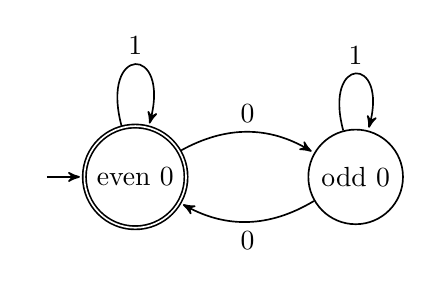
\begin{tikzpicture}[->,>=stealth',shorten >=1pt,auto,node distance=2.8cm,semithick]
\node[state,initial,initial text=,accepting] (n1) {even $0$};
\node[state] (n2) [right of=n1] {odd $0$};

\path[->](n1) edge[loop above] node[above] {$1$} ();
\path[->](n2) edge[loop above] node[above] {$1$} ();

\path[->](n1) edge[bend left] node[above] {$0$} (n2);
\path[->](n2) edge[bend left] node[below] {$0$} (n1);
\end{tikzpicture}
\Img{GI(U)-16.04.2009-IMG-2}

$L_1 = \gklamm{w \in \Sigma_{\tx{Bool}}^* \vert \betrag{w}_0 \tx{ gerade } \und \betrag{w}_1 \tx{ gerade}}$

\Insert{GI(U)-16.04.2009-IMG-3}

$L_2 = \gklamm{w \in \Sigma_{\tx{Bool}}^* \vert \betrag{w}_0 \tx{ gerade } \und \betrag{w}_1 \tx{ gerade} \oder \betrag{w}_0 \tx{ gerade } \und \betrag{w}_1 \tx{ ungerade}}$

\Insert{GI(U)-16.04.2009-IMG-4}

$L_3 = \gklamm{w \in \Sigma_{\tx{Bool}}^* \vert Zahlenwert (w) \mod 4 = 0}$
$\approx \gklamm{w \in \Sigma_{\tx{Bool}}^* \vert w \tx{ endet auf } 00}$
Erstmal: $w$ beginnt mit $00$

\Insert{GI(U)-16.04.2009-IMG-5}

\Insert{GI(U)-16.04.2009-IMG-6}

$L_4 = \gklamm{w \in \Sigma_{\tx{Bool}}^* \vert w \tx{ enth�lt } 110110}$

\Insert{GI(U)-16.04.2009-IMG-7}

\section{Tutorium}
\subsection{Aufgaben}
\subsubsection{Vom 21.04.2009}
\begin{enumerate}
\item $L_1 \gklamm{w \in \Sigma_{\tx{Bool}}^* \vert \betrag{w}_1 \mod 2 = 0 \und \betrag{w}_0 = 1}$
\item $L_2 \gklamm{w \in \Sigma_{\tx{Bool}}^* \vert w \tx{ enth�lt } 101101}$
\item $L_3 \gklamm{w \in \Sigma_{\tx{Bool}}^* \vert w \tx{ enth�lt mindestens zweimal } 0}$
\item $L_4 \gklamm{w \in \Sigma_{\tx{Bool}}^* \vert w 0 v \und v \tx{ enth�lt gerade Anzahl an 1en}}$
\end{enumerate}

\subsection{L�sungen}
\subsubsection{Vom 21.04.2009}
\begin{enumerate}
\item L�sung siehe Abbildung \vref{fig:Tutorium_22_01_2009_1}.
		\begin{figure}[htb]
		\centering
		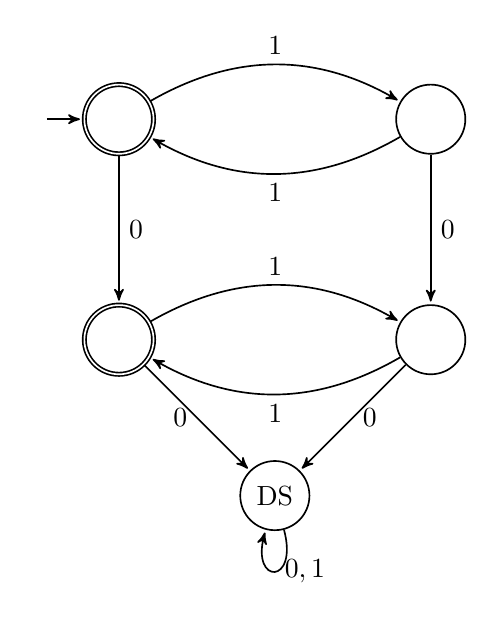
\begin{tikzpicture}[->,>=stealth',shorten >=1pt,auto,node distance=2.8cm,semithick]
		\node[state]
		(node5) 									{DS};
		\node[state,accepting]
		(node3) [above left of=node5] 	{};
		\node[state]
		(node4) [above right of=node5] 	{};
		\node[state,initial,accepting,initial text=]
		(node1) [above of=node3]			{};
		\node[state]
		(node2) [above of=node4] 			{};
		
		\path[->] (node1) edge [bend left] node[above] {$1$} (node2);
		\path[->] (node2) edge [bend left] node[below] {$1$} (node1);
		\path[->] (node1) edge node[right] {$0$} (node3);
		\path[->] (node2) edge node[right] {$0$} (node4);
		\path[->] (node3) edge [bend left] node[above] {$1$} (node4);
		\path[->] (node4) edge [bend left] node[below] {$1$} (node3);
		\path[->] (node3) edge node[left] {$0$} (node5);
		\path[->] (node4) edge node[right] {$0$} (node5);
		\path[->] (node5) edge [loop below] node[right] {$0,1$} ();
		\end{tikzpicture}
		\caption{L�sung zu $L_1$}
		\label{fig:Tutorium_22_01_2009_1}
		\end{figure}

\item L�sung siehe Abbildung \vref{fig:Tutorium_22_01_2009_2}.
		\begin{figure}[htb]
		\centering
		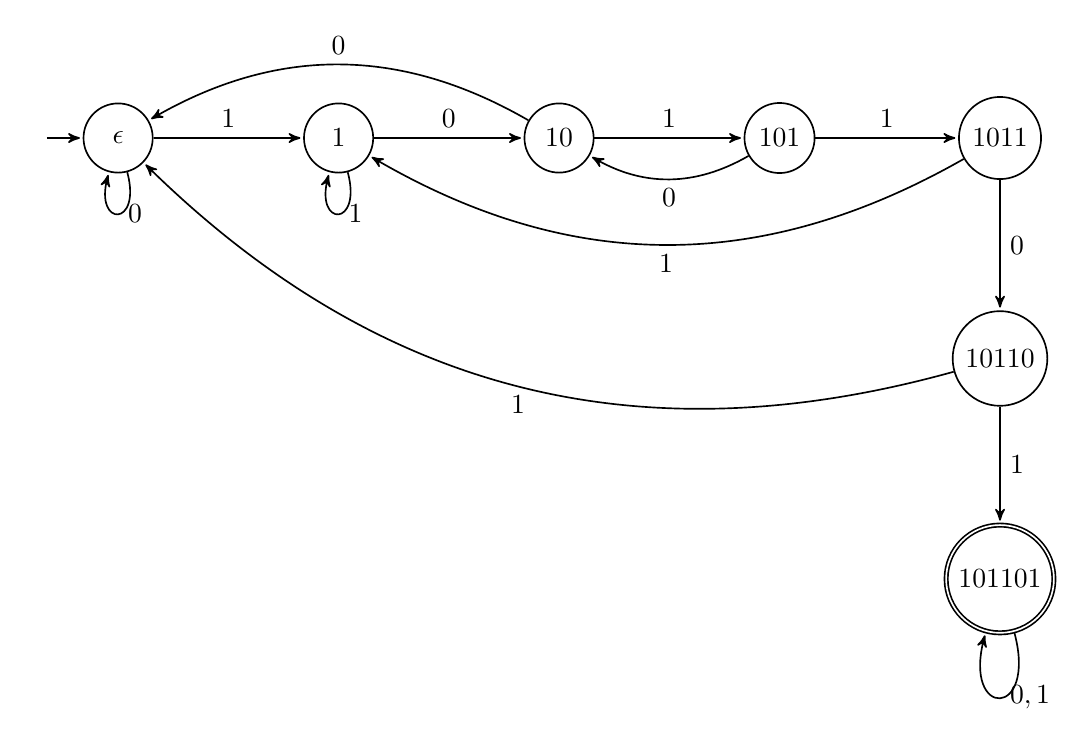
\begin{tikzpicture}[->,>=stealth',shorten >=1pt,auto,node distance=2.8cm,semithick]
		\node[state,initial, initial text=] (n1) {$\epsilon$};
		\node[state] (n2) [right of=n1] {$1$};
		\node[state] (n3) [right of=n2] {$10$};
		\node[state] (n4) [right of=n3] {$101$};
		\node[state] (n5) [right of=n4] {$1011$};
		\node[state] (n6) [below of=n5] {$10110$};
		\node[state,accepting] (n7) [below of=n6] {$101101$};
		
		\path[->] (n1) edge node[above] {$1$} (n2);
		\path[->] (n2) edge node[above] {$0$} (n3);
		\path[->] (n3) edge node[above] {$1$} (n4);
		\path[->] (n4) edge node[above] {$1$} (n5);
		\path[->] (n5) edge node[right] {$0$} (n6);
		\path[->] (n6) edge node[right] {$1$} (n7);
		
		\path[->] (n1) edge [loop below] node[right] {$0$} ();
		\path[->] (n2) edge [loop below] node[right] {$1$} ();
		\path[->] (n3) edge [bend right] node[above] {$0$} (n1);
		\path[->] (n4) edge [bend left] node[below] {$0$} (n3);
		\path[->] (n5) edge [bend left] node[below] {$1$} (n2);
		\path[->] (n6) edge [bend left] node[below] {$1$} (n1);
		\path[->] (n7) edge [loop below] node[right] {$0,1$} ();
		\end{tikzpicture}
		\caption{L�sung zu $L_2$}
		\label{fig:Tutorium_22_01_2009_2}
		\end{figure}

\item L�sung siehe Abbildung \vref{fig:Tutorium_22_01_2009_3}.
		\begin{figure}[htb]
		\centering
		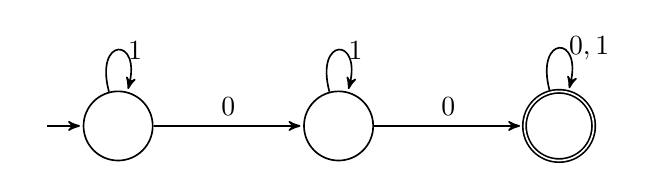
\begin{tikzpicture}[->,>=stealth',shorten >=1pt,auto,node distance=2.8cm,semithick]
		\node[state,initial,initial text=] (n1) {};
		\node[state] (n2) [right of=n1] {};
		\node[state,accepting] (n3) [right of=n2] {};
		
		\path[->] (n1) edge node[above] {$0$} (n2);
		\path[->] (n2) edge node[above] {$0$} (n3);
		
		\path[->] (n1) edge [loop above] node[right] {$1$} ();
		\path[->] (n2) edge [loop above] node[right] {$1$} ();
		\path[->] (n3) edge [loop above] node[right] {$0,1$} ();
		\end{tikzpicture}
		\caption{L�sung zu $L_3$}
		\label{fig:Tutorium_22_01_2009_3}
\end{figure}
\end{enumerate}

\section{2. �bung}
\subsection{1. Aufgabe}
\begin{enumerate}[label=(\alph*)]
\item \begin{enumerate}[label=\arabic*)]
		\item ohne Gewicht
				\begin{itemize}
				\item Eintr�ge in der Adjazenzmatrix: 1 oder 0
				\item Trennzeichen nicht n�tig da Adjazenzmatrix quadratisch
						\begin{itemize}[label=$\hookrightarrow$]
						\item 2\,$\times$ durch String laufen n�tig um Adjazenzmatrix zu rekonstruieren
						\end{itemize}
						Alternative Kodierung: $0$ durch $00$ $1$ durch 01 $\sharp$ durch $11$
				\end{itemize}

		\item mit Gewicht
				\begin{itemize}
				\item in Adjazenzmatrix: Gewichte (\ac{z.B.} nat�rliche Zahlen)
				\item Zahl $n$ kodieren durch $n$-maliges hintereinander schreiben der $0$, $1$ als Trennzeichen
				\end{itemize}
		\end{enumerate}

\item Graph ohne Gewicht einfach alle Zeilen hintereinander schreiben
		\begin{itemize}[label=$\hookrightarrow$]
		\item neue L�nge $n^2$ anstelle von $n^2 + n$
		\item Trennzeichen nicht n�tig
		\end{itemize}
\end{enumerate}

\subsection{2. Aufgabe}
Trivial! Schon Gemacht!

\subsection{3. Aufgabe}
\Todo{von meiner L�sung nachtragen}

\subsection{4. Aufgabe}
\Todo{von meiner L�sung nachtragen}

\subsection{5. Aufgabe}
unendliche Menge von W�rtern $y_1, y_2, \dots$ mit $\betrag{y_i} < \betrag{y_{i + 1}}$ f�r i = $1, 2, 3, \dots$ $\exists c$, so dass gilt
\[KC(y_i) \klgl \lceil \ld \ld \ld \betrag{y_i}\rceil + c\]
$y_i = 1^{2^{2^i}}$\\
$\betrag{y_i} = 2^{2^i}$, $\betrag{y_{i + 1}} = 2^{2^{i + 1}}$ \Ra $\underbrace{2^{2^i} < 2^{2^i}}_{\tx{f�r alle } i \in \mb{N}}$
\Insert{GI(T)-05.05.2009-LST-1}
Darstellung von $i \ra \lceil \ld i \rceil$ Bits\\
$KC(y_i) \klgl \lceil \ld i \rceil + c = \lceil \ld \ld \ld \betrag{y_i} \rceil + c$

%</Text>%%%%%%%%%%%%%%%%%%%%%%%%%%%%%%%%%%%%%%%%%%%%%%%%%%%%%%%%%%%%%%%%%%%%%%%
\backmatter
%Literaturverzeichnis
%\newpage
%\addcontentsline{toc}{part}{Literaturverzeichnis}
%\bibliography{literatur}{}

%Stichwortverzeichnis
\newpage
\renewcommand{\indexname}{Stichwortverzeichnis}
\addcontentsline{toc}{part}{Stichwortverzeichnis}
\printindex

\end{document}
